\documentclass[tikz, border=20pt]{standalone}
\usepackage{helvet}
\renewcommand{\familydefault}{\sfdefault}
\usetikzlibrary{arrows.meta, calc}

\tikzset{
    entity/.style={rectangle, draw=black, line width=1.8pt, fill=white,
        text width=2.8cm, align=center, minimum height=1.3cm, font=\small\bfseries},
    process/.style={circle, draw=black, line width=1.5pt, fill=white,
        minimum size=2.8cm, align=center, font=\scriptsize\bfseries},
    arr/.style={->, line width=1pt, >=stealth, draw=black},
    feedback/.style={->, line width=1pt, >=stealth, draw=black, dashed},
    lbl/.style={font=\scriptsize, fill=white, inner sep=2pt, align=center, text width=2.2cm}
}
\newcommand{\datastore}[3]{%
    \node[rectangle, draw=none, fill=white, text width=3.0cm,
          align=center, minimum height=0.9cm, font=\scriptsize\bfseries] (#1) at #2 {#3};
    \draw[line width=1.2pt] (#1.north west) -- (#1.north east);
    \draw[line width=1.2pt] (#1.south west) -- (#1.south east);
    \draw[line width=1.2pt] (#1.north west) -- (#1.south west);
    \draw[line width=1.2pt] (#1.north east) -- (#1.south east);
}

\begin{document}
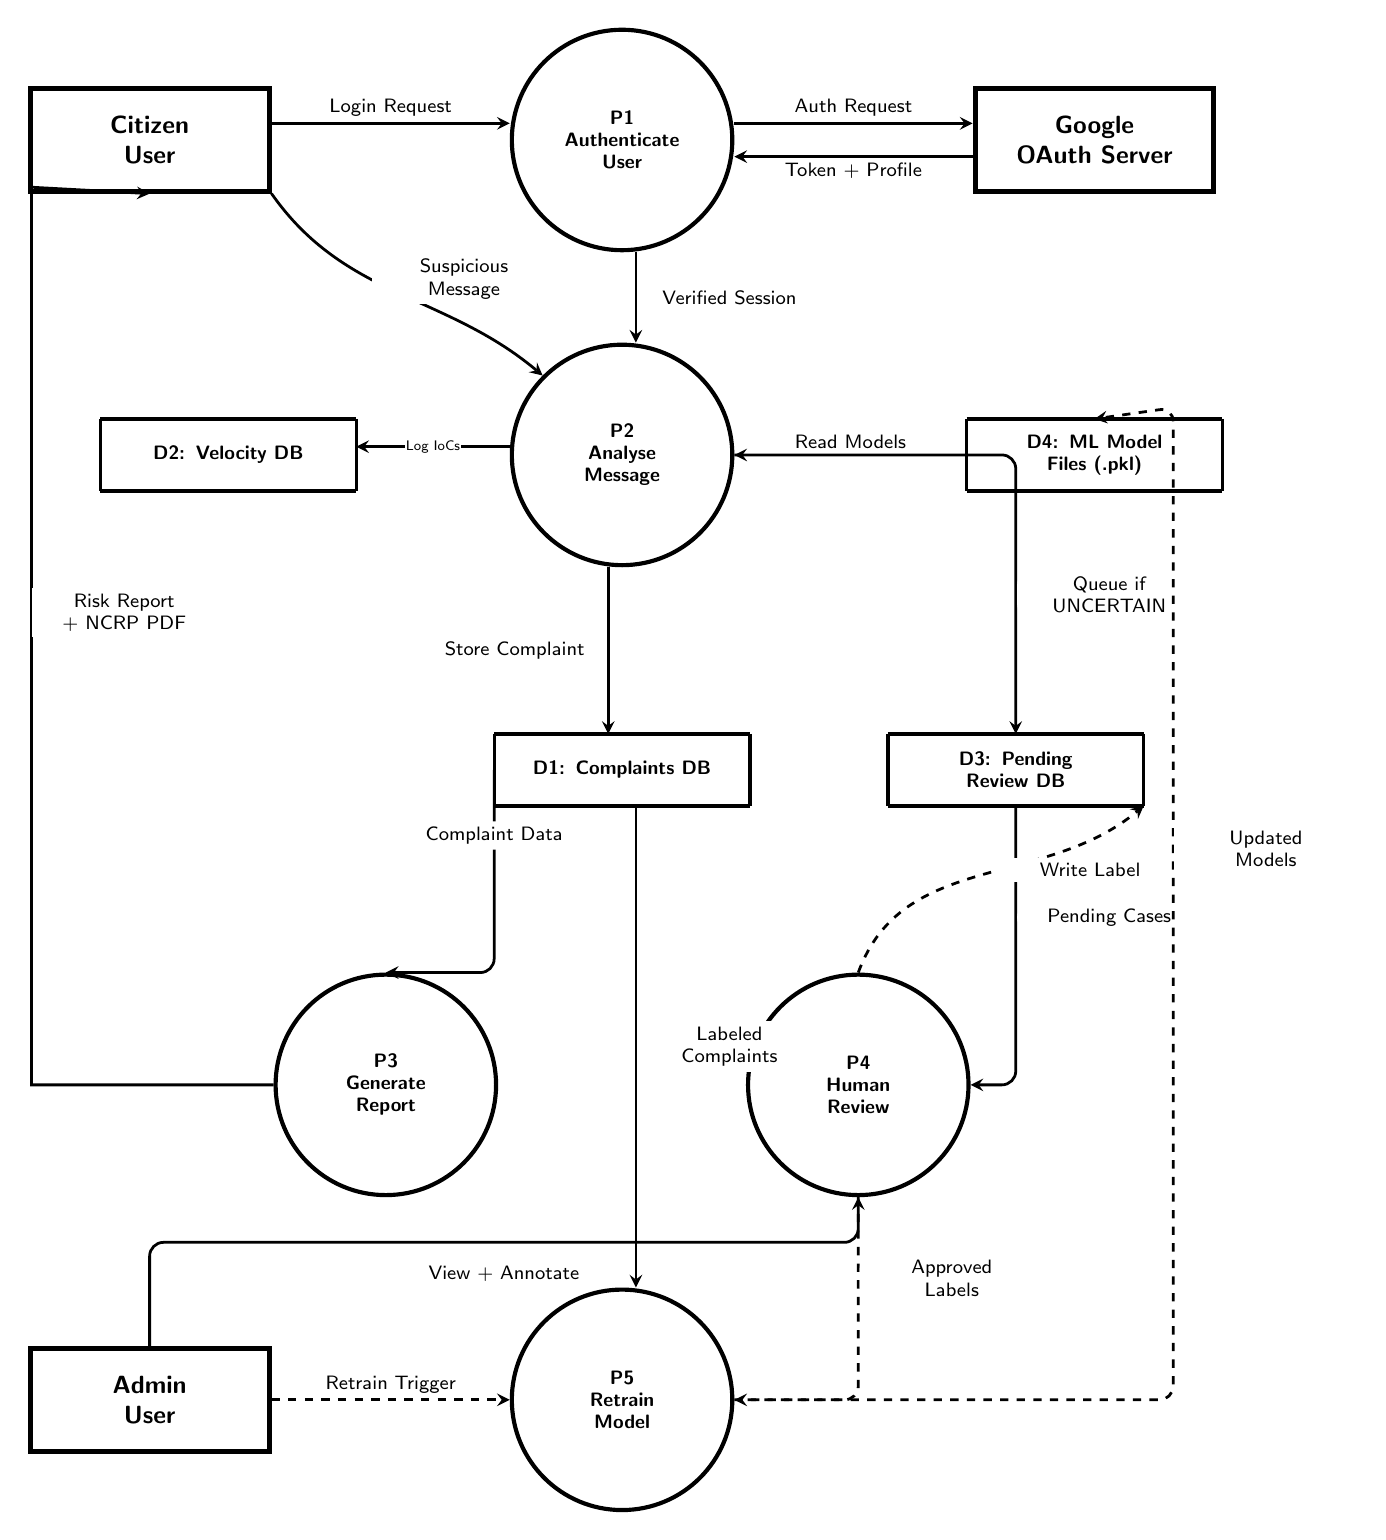
\begin{tikzpicture}
%% LAYOUT:
%% y= 9: Citizen(-6,9)  P1(0,9)   OAuth(6,9)
%% y= 5: D2(-5,5)       P2(0,5)   D4(6,5)
%% y= 1:                D1(0,1)   D3(5,1)   <-- D3 moved to x=5
%% y=-3: P3(-3,-3)      P4(3,-3)  <-- P4 moved to x=3
%% y=-7: Admin(-6,-7)   P5(0,-7)

\node[entity]  (citizen) at (-6,  9) {Citizen\\User};
\node[entity]  (admin)   at (-6, -7) {Admin\\User};
\node[entity]  (oauth)   at ( 6,  9) {Google\\OAuth Server};
\node[process] (p1) at (0,  9)  {\textbf{P1}\\Authenticate\\User};
\node[process] (p2) at (0,  5)  {\textbf{P2}\\Analyse\\Message};
\node[process] (p3) at (-3, -3) {\textbf{P3}\\Generate\\Report};
\node[process] (p4) at ( 3, -3) {\textbf{P4}\\Human\\Review};
\node[process] (p5) at ( 0, -7) {\textbf{P5}\\Retrain\\Model};

\datastore{d1}{(0,  1)}{D1: Complaints DB}
\datastore{d2}{(-5, 5)}{D2: Velocity DB}
\datastore{d3}{(5,  1)}{D3: Pending\\Review DB}
\datastore{d4}{(6,  5)}{D4: ML Model\\Files (.pkl)}

%% ── P1: AUTHENTICATION ──────────────────────────────────────────
\draw[arr]
    ([yshift=6pt]citizen.east) --
    node[lbl,above]{Login Request}
    ([yshift=6pt]p1.west);

\draw[arr]
    ([yshift=6pt]p1.east) --
    node[lbl,above]{Auth Request}
    ([yshift=6pt]oauth.west);

\draw[arr]
    ([yshift=-6pt]oauth.west) --
    node[lbl,below]{Token + Profile}
    ([yshift=-6pt]p1.east);

\draw[arr]
    ([xshift=5pt]p1.south) --
    node[lbl,right]{Verified Session}
    ([xshift=5pt]p2.north);

%% ── P2: ANALYSE ─────────────────────────────────────────────────
%% Citizen → P2: diagonal arc (avoids D2 at same y)
\draw[arr]
    (citizen.south east)
    to[out=305, in=140]
    node[lbl,right,pos=0.4]{Suspicious\\Message}
    (p2.north west);

\draw[arr] ([yshift=3pt]p2.west) --
    node[font=\tiny, fill=white, inner sep=0.5pt, align=center]{Log IoCs}
    ([yshift=3pt]d2.east);
\draw[arr] (d4.west) -- node[lbl,above]{Read Models} (p2.east);

\draw[arr]
    ([xshift=-5pt]p2.south) --
    node[lbl,left]{Store Complaint}
    ([xshift=-5pt]d1.north);

%% P2 → D3: right then down
\draw[arr, rounded corners=5pt]
    (p2.east) -|
    node[lbl,right,pos=0.75]{Queue if\\UNCERTAIN}
    (d3.north);

%% ── P3: REPORT ──────────────────────────────────────────────────
%% D1 → P3: left then down
\draw[arr, rounded corners=5pt]
    (d1.west) |-
    node[lbl,above,pos=0.2]{Complaint Data}
    (p3.north);

%% P3 → Citizen: up far-left border at x=-7.5, arrive at citizen.south
\draw[arr]
    (p3.west) -- (-7.5,-3) -- (-7.5,8.4) -- (citizen.south);
\node[lbl,right] at (-7.5,3) {Risk Report\\+ NCRP PDF};

%% ── P4: HUMAN REVIEW ────────────────────────────────────────────
%% Admin → P4: from admin.north, up to y=-5, right to P4.south
\draw[arr, rounded corners=5pt]
    (admin.north) -- (-6,-5) -- (3,-5) -- (p4.south);
\node[lbl] at (-1.5,-5.4) {View + Annotate};

%% D3 → P4 (Pending Cases): down from D3, left to P4 east side
%% Route at y=-3: d3.south -> down to y=-3, left to p4
\draw[arr, rounded corners=5pt]
    (d3.south) |-
    node[lbl,right,pos=0.2]{Pending Cases}
    (p4.east);

%% P4 → D3 (Write Label, dashed): tight arc, stays within diagram
\draw[feedback]
    (p4.north)
    to[out=70, in=220]
    node[lbl,right,pos=0.55]{Write Label}
    (d3.south east);

%% ── P5: RETRAIN ─────────────────────────────────────────────────
%% P4 → P5 (Approved Labels, dashed): down then left
\draw[feedback, rounded corners=5pt]
    (p4.south) |-
    node[lbl,right,pos=0.2]{Approved\\Labels}
    (p5.east);

%% Admin → P5 (Retrain Trigger, dashed): straight right same y=-7
\draw[feedback]
    (admin.east) --
    node[lbl,above]{Retrain Trigger}
    (p5.west);

%% D1 → P5 (Labeled Complaints): straight down right offset
\draw[arr]
    ([xshift=5pt]d1.south) --
    node[lbl,right]{Labeled\\Complaints}
    ([xshift=5pt]p5.north);

%% P5 → D4 (Updated Models, dashed): right border at x=7, arrive at d4.north
\draw[feedback, rounded corners=5pt]
    (p5.east) -- (7,-7) -- (7,5.6) -- (d4.north);
\node[lbl,right] at (7,0) {Updated\\Models};

\end{tikzpicture}
\end{document}
